\section{Conduction Through The Walls}\label{conduction-through-the-walls}

\subsection{Conduction Transfer Function Module}\label{conduction-transfer-function-module}

The most basic time series solution is the response factor equation which relates the flux at one surface of an element to an infinite series of temperature histories at both sides as shown by Equation~\ref{eq:BaseResponseFactorEquation}:

\begin{equation}
{q''_{ko}}(t) = \sum\limits_{j = 0}^\infty  {{X_j}} {T_{o,t - j\delta }} - \sum\limits_{j = 0}^\infty  {{Y_j}} {T_{i,t - j\delta }}
\label{eq:BaseResponseFactorEquation}
\end{equation}

where q'' is heat flux, T is temperature, i signifies the inside of the building element, o signifies the outside of the building element, t represents the current time step, and X and Y are the response factors.

While in most cases the terms in the series decay fairly rapidly, the infinite number of terms needed for an exact response factor solution makes it less than desirable.~ Fortunately, the similarity of higher order terms can be used to replace them with flux history terms.~ The new solution contains elements that are called conduction transfer functions (CTFs).~ The basic form of a conduction transfer function solution is shown by the following equation:

\begin{equation}
{q''_{ki}}(t) =  - {Z_o}{T_{i,t}} - \sum\limits_{j = 1}^{nz} {{Z_j}} {T_{i,t - j\delta }} + {Y_o}{T_{o,t}} + \sum\limits_{j = 1}^{nz} {{Y_j}} {T_{o,t - j\delta }} + \sum\limits_{j = 1}^{nq} {{\Phi_j}{{q''}_{ki,t - j\delta }}}
\end{equation}

for the inside heat flux, and

\begin{equation}
{q''_{ko}}(t) =  - {Y_o}{T_{i,t}} - \sum\limits_{j = 1}^{nz} {{Y_j}} {T_{i,t - j\delta }} + {X_o}{T_{o,t}} + \sum\limits_{j = 1}^{nz} {{X_j}} {T_{o,t - j\delta }} + \sum\limits_{j = 1}^{nq} {{\Phi_j}{{q''}_{ko,t - j\delta }}}
\end{equation}

for the outside heat flux (q'' = q/A)

where:

X\emph{\(_{j}\)} ~ = Outside CTF coefficient, j = 0,1,\ldots{}nz.

Y\emph{\(_{j}\)} = Cross CTF coefficient, j = 0,1,\ldots{}nz.

Z\emph{\(_{j}\)} = Inside CTF coefficient, j = 0,1,\ldots{}nz.

$\Phi$\emph{\(_{j}\)} = Flux CTF coefficient, j = 1,2,\ldots{}nq.

T\emph{\(_{i}\)} = Inside face temperature

T\emph{\(_{o}\)} = Outside face temperature

\({q''_{ko}}\) ~ = Conduction heat flux on outside face

\(q''\) ~ = Conduction heat flux on inside face

The subscript following the comma indicates the time period for the quantity in terms of the time step (\(\delta\)).~ Note that the first terms in the series (those with subscript 0) have been separated from the rest in order to facilitate solving for the current temperature in the solution scheme.~ These equations state that the heat flux at either face of the surface of any generic building element is linearly related to the current and some of the previous temperatures at both the interior and exterior surface as well as some of the previous flux values at the interior surface.

The final CTF solution form reveals why it is so elegant and powerful.~ With a single, relatively simple, linear equation with constant coefficients, the conduction heat transfer through an element can be calculated.~ The coefficients (CTFs) in the equation are constants that only need to be determined once for each construction type.~ The only storage of data required are the CTFs themselves and a limited number of temperature and flux terms.~ The formulation is valid for any surface type and does not require the calculation or storage of element interior temperatures.

\subsection{Calculation of Conduction Transfer Functions}\label{calculation-of-conduction-transfer-functions}

The basic method used in EnergyPlus for CTF calculations is known as the state space method (Ceylan and Myers 1980; Seem 1987; Ouyang and Haghighat 1991).~ Another common, older method used Laplace transformations to reach the solution;~ the Laplace method was~ used in BLAST (Hittle, 1979; Hittle \& Bishop, 1983).~ The basic state space system is defined by the following linear matrix equations:

\begin{equation}
\frac{{d\left[ {\bf{x}} \right]}}{{dt}} = \left[ {\bf{A}} \right]\left[ {\bf{x}} \right] + \left[ {\bf{B}} \right]\left[ {\bf{u}} \right]
\end{equation}

\begin{equation}
\left[ {\bf{y}} \right] = \left[ {\bf{C}} \right]\left[ {\bf{x}} \right] + \left[ {\bf{D}} \right]\left[ {\bf{u}} \right]
\end{equation}

where x is a vector of state variables, u is a vector of inputs, y is the output vector, t is time, and A, B, C, and D are coefficient matrices.~ Through the use of matrix algebra, the vector of state variables (x) can be eliminated from the system of equations, and the output vector (y) can be related directly to the input vector (u) and time histories of the input and output vectors.

This formulation can be used to solve the transient heat conduction equation by enforcing a finite difference grid over the various layers in the building element being analyzed.~ In this case, the state variables are the nodal temperatures, the environmental temperatures (interior and exterior) are the inputs, and the resulting heat fluxes at both surfaces are the outputs.~ Thus, the state space representation with finite difference variables would take the following form:

\begin{equation}
\frac{d\left[\begin{array}{c}T_1 \\ \vdots \\ T_n\end{array}\right]}{dt} = \left[\bf{A}\right]\left[\begin{array}{c}T_1 \\ \vdots \\ T_n\end{array}\right]+\left[\bf{B}\right]\left[\begin{array}{c}T_i \\ T_o\end{array}\right]
\end{equation}

\begin{equation}
\left[\begin{array}{c}{q''}_i \\ {q''}_o\end{array}\right] = \left[\bf{C}\right]\left[\begin{array}{c}T_1 \\ \vdots \\ T_n\end{array}\right]+\left[\bf{D}\right]\left[\begin{array}{c}T_i \\ T_o\end{array}\right]
\end{equation}

where T1, T2, \ldots{}, Tn-1, Tn~are the finite difference nodal temperatures, n is the number of nodes, Ti~and To~are the interior and exterior environmental temperatures, and q``i~and q''o~are the heat fluxes (desired output).

Seem (1987) shows that for a simple one layer slab with two interior nodes as in Figure~\ref{fig:two-node-state-space-example.} and convection at both sides the resulting finite difference equations are given by:

\begin{equation}
C\frac{{d{T_1}}}{{dt}} = hA\left( {{T_o} - {T_1}} \right) + \frac{{{T_2} - {T_1}}}{R}
\end{equation}

\begin{equation}
C\frac{{d{T_2}}}{{dt}} = hA\left( {{T_i} - {T_2}} \right) + \frac{{{T_1} - {T_2}}}{R}
\end{equation}

\begin{equation}
q{``_i} = h\left( {{T_i} - {T_2}} \right)
\end{equation}

\begin{equation}
q{``_o} = h\left( {{T_1} - {T_o}} \right)
\end{equation}

where:

\(R = \frac{\ell }{{kA}}\) ,

\(C = \frac{{\rho {c_p}\ell A}}{2}\) , and

A is the area of the surface exposed to the environmental temperatures.

In matrix format:

\begin{equation}
\left[\begin{array}{c}\frac{dT_1}{dt} \\ \frac{dT_2}{dt}\end{array}\right] = 
     \left[\begin{array}{cc}-\frac{1}{RC}-\frac{hA}{C} & \frac{1}{RC} \\ \frac{1}{RC} & -\frac{1}{RC}-\frac{hA}{C}\end{array}\right]\left[\begin{array}{c}T_1 \\ T_2\end{array}\right] + 
     \left[\begin{array}{cc}\frac{hA}{C} & 0 \\ 0 & \frac{hA}{C}\end{array}\right]\left[\begin{array}{c}T_o \\ T_i\end{array}\right]
\end{equation}

\begin{equation}
\left[\begin{array}{c}{q''}_o \\ {q''}_i\end{array}\right] = 
    \left[\begin{array}{cc}0 & -h \\ h & 0\end{array}\right] \left[\begin{array}{c}T_1 \\ T_2\end{array}\right] +
    \left[\begin{array}{cc}0 & h \\ -h & 0\end{array}\right] \left[\begin{array}{c}T_o \\ T_i\end{array}\right]
\end{equation}

\begin{figure}[hbtp] % fig 10
\centering
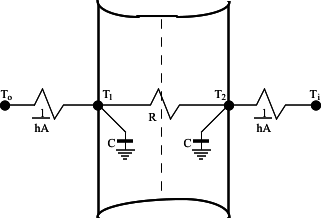
\includegraphics[width=0.9\textwidth, height=0.9\textheight, keepaspectratio=true]{media/image168.svg.png}
\caption{Two Node State Space Example. \protect \label{fig:two-node-state-space-example.}}
\end{figure}

The important aspect of the state space technique is that through the use of matrix algebra the state space variables (nodal temperatures) can be eliminated to arrive at a matrix equation that gives the outputs (heat fluxes) as a function of the inputs (environmental temperatures) only.~ This eliminates the need to solve for roots in the Laplace domain.~ In addition, the resulting matrix form has more physical meaning than complex functions required by the Laplace transform method.

The accuracy of the state space method of calculating CTFs has been addressed in the literature.~ Ceylan and Myers (1980) compared the response predicted by the state space method to various other solution techniques including an analytical solution.~ Their results showed that for an adequate number of nodes the state space method computed a heat flux at the surface of a simple one layer slab within 1\% of the analytical solution.~ Ouyang and Haghighat (1991) made a direct comparison between the Laplace and state space methods.~ For a wall composed of insulation between two layers of concrete, they found almost no difference in the response factors calculated by each method.

Seem (1987) summarizes the steps required to obtain the CTF coefficients from the A, B, C, and D matrices.~ While more time consuming than calculating CTFs using the Laplace Transform method, the matrix algebra (including the calculation of an inverse and exponential matrix for A) is easier to follow than root find algorithms.~ Another difference between the Laplace and State Space methods is the number of coefficients required for a solution.~ In general, the State Space method requires more coefficients.~ In addition, the number of temperature and flux history terms is identical (nz = nq).~ Note that as with the Laplace method that the actual number of terms will vary from construction to construction.

Two distinct advantages of the State Space method over the Laplace method that are of interest when applying a CTF solution for conduction through a building element are the ability to obtain CTFs for much shorter time steps and the ability to obtain 2- and 3-D conduction transfer functions.~ While not implemented in the Toolkit, both Seem (1987) and Strand (1995) have demonstrated the effectiveness of the State Space method in handling these situations that can have important applications in buildings.

\subsection{Conduction Transfer Function (CTF) Calculations in EnergyPlus}\label{conduction-transfer-function-ctf-calculations-in-energyplus}

Conduction transfer functions are an efficient method to compute surface heat fluxes because they eliminate the need to know temperatures and fluxes within the surface.~ However, conduction transfer function series become progressively more unstable as the time step decreases.~ This became a problem as investigations into short time step computational methods for the zone/system interactions progressed because, eventually, this instability caused the entire simulation to diverge.~ This phenomenon was most apparent for thermally massive constructions with long characteristic times and, correspondingly, requiring a large number of terms in the CTF series. This indicates that the problem is related to round-off and truncation error and is in no way an indictment of the CTF method itself.~ Methods that develop CTF series from finite difference approximations to the heat conduction equation (Meyers, 1980; Seem, 1987) were considered to address this problem.~ Seem's method did give better accuracy and stability at short time steps than the current BLAST technique but, the method still had difficulty computing stable CTF series for time steps of less than 1/4 hour for the heaviest constructions in the BLAST library.

The zone heat gains consist of specified internal heat gains, air exchange between zones, air exchange with the outside environment, and convective heat transfer from the zone surfaces.~ Of these, the surface convection load requires the most complicated calculations because a detailed energy balance is required at the inside and outside surface of each wall, floor, and roof.~ In addition, the transient heat conduction in the material between the surfaces must be solved.~ This solution gives the inside and outside temperatures and heat fluxes that must be known in order to calculate the convection component to the zone load for each zone surface.~ BLAST uses a conduction transfer function CTF method attributed to Hittle (1980) to solve the transient conduction problem for each surface.~ The method results in a time series of weighting factors that, when multiplied by previous values of the surface temperatures and fluxes and the current inside and outside surface temperatures, gives the current inside and outside heat flux.~ The method is easily applied to multilayered constructions for which analytical solutions are unavailable.~ In addition, determining the series of CTF coefficients is a one-time calculation, making the method much faster than finite difference calculations.

A problem with CTF methods is that the series time step is fixed; that is, a CTF series computed for a one hour time step takes information at t-1 hours, t-2 hours, etc. and computes conditions at the current time t.~ As time advances the oldest term in the input series is dropped and the data moved back one time step to allow the newest value to be added to the series.~ For convenience, the time step used to determine the CTF series should be the same as the time step used to update the zone mean air temperature in the zone energy balance.~ But, as the time step used to calculate the CTF series gets shorter, the number of terms in the series grows.~ Eventually, with enough terms, the series becomes unstable due to truncation and round-off error.~ Heavy constructions, such as slab-on-grade floors (12" heavyweight concrete over 18" dirt), have accuracy and stability problems at time steps as large as 0.5 hours when modeled by Hittle's CTF method.~ In an attempt to overcome this problem, Hittle's method was replaced by Seem's method (1987) in IBLAST.~ This resulted in some improvement in stability at shorter time steps, but not enough to allow IBLAST to run at a 0.1 hour time step without restricting the types of surfaces that could be used.

Even though CTF methods require that values of the surface temperatures and fluxes be stored for only a few specific times before the current time, the temperature and flux histories are, actually, continuous functions between those discrete points.~ However, there is no way to calculate information at these intermediate times once a series has been initialized.~ The terms in the temperature and flux histories are out of phase with these points.~ However, they can be calculated by shifting the phase of the temperature and flux histories by only a fraction of a time step.~ This procedure would allow a CTF series computed for a time step Dt, to be used to compute information at times t+Dt/2, t+Dt/3, t+Dt/4, or any other arbitrary fraction of the time step, so long as the surface temperatures and flux values were still Dt apart.~ Several ways of doing this are described below.

The method shown in the Figure~\ref{fig:multiple-staggered-time-history-scheme} maintains two sets of histories out of phase with each other.~ The figure shows how this would work for two sets of histories out of phase by one half of a time step.~ More sets of temperature and flux histories could be used, allowing the simulation time step to take on values: 1/3, 1/4, 1/5, etc., of the minimum time step allowed for the CTF calculations.~ The time step between inputs to the CTF series would be the smallest convenient interval at which the CTF series is stable.~ This scenario is illustrated in this figure for two separate sets of temperature and flux histories.~ Cycling through each history, in order, allowed calculations of the zone energy balance to be performed with updated surface information at a shorter time step than one CTF history series would otherwise allow.~ This method required no interpolation between the series once each set of histories was initialized.~ However, if the smallest time step for a stable CTF series was large compared to the zone temperature update time step, significant memory was required to store all the sets of histories.

\begin{figure}[hbtp] % fig 11
\centering
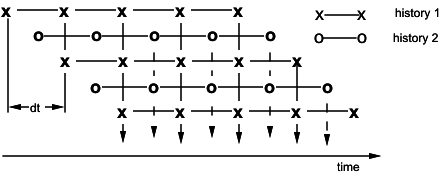
\includegraphics[width=0.9\textwidth, height=0.9\textheight, keepaspectratio=true]{media/image169.svg.png}
\caption{Multiple, staggered time history scheme \protect \label{fig:multiple-staggered-time-history-scheme}}
\end{figure}

Another method is shown in Figure~\ref{fig:sequential-interpolation-of-new-histories}. Sequential interpolation of new histories that uses successive interpolations to determine the next set of temperature and flux histories.~ The current history is interpolated directly from the previous history set using the required time phase shift between the two.~ This method required permanent storage for only one set of temperature and flux histories at a time, but smoothed out temperature and flux data as more interpolations were performed.~ As a result, at concurrent simulation times current values of history terms were different form previous ``in phase'' history terms.~ This was unacceptable from, a physical point of view, because it allowed current information to change data from a previous time.

\begin{figure}[hbtp] % fig 12
\centering
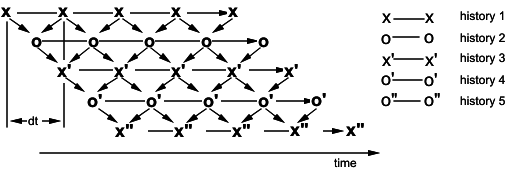
\includegraphics[width=0.9\textwidth, height=0.9\textheight, keepaspectratio=true]{media/image170.svg.png}
\caption{Sequential interpolation of new histories \protect \label{fig:sequential-interpolation-of-new-histories}}
\end{figure}

A final method, shown in Figure~\ref{fig:master-history-with-interpolation}. Master history with interpolation, was something of a hybrid of the previous two methods.~ One ``master'' history set was maintained and updated for all time; this solved the problem of current events propagating information backwards in time.~ When surface fluxes needed to be calculated at times out of phase with this master history a new, temporary history was interpolated from the master values.~ This method proved to be the best of the three options described because it eliminated propagation of information backwards in time and only required concurrent storage of two sets of temperature and flux histories. This method was subsequently incorporated into the IBLAST program in conjunction with Seem's procedure for calculating the coefficients of the CTF series.

\begin{figure}[hbtp] % fig 13
\centering
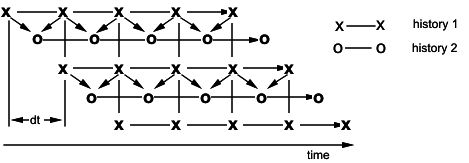
\includegraphics[width=0.9\textwidth, height=0.9\textheight, keepaspectratio=true]{media/image171.svg.png}
\caption{Master history with interpolation \protect \label{fig:master-history-with-interpolation}}
\end{figure}

\subsection{Conduction Transfer Function (CTF) Calculations Special Case: R-Value Only Layers}\label{conduction-transfer-function-ctf-calculations-special-case-r-value-only-layers}

Most users will elect to enter materials with four parameters that are of interest for calculating conduction transfer functions: thickness, conductivity, density, and specific heat.~ For these materials, EnergyPlus will divide each material layer within a construction into between 6 and 18 nodes for the application of the state-space method.~ For multi-layered constructions, nodes are also placed at the interface between two layers.~ These interface nodes consist of half a node of the first layer and half a node of the second layer.

In some cases, either due to a lack of information or a desire to simplify input, a user may choose to enter a material layer as a ``no mass'' or ``R-Value only'' material.~ This assumption essentially says that these layers add nothing to the thermal mass of the overall construction and only add to the overall resistance or R-Value of the construction as a whole.~ While this is not recommended, it is allowed and in some cases is not a poor assumption for extremely lightweight materials such as some types of insulation.

In the past, when a user enters such a ``no mass'' material into EnergyPlus, internally the properties of this layer are converted to approximate the properties of air (density, specific heat, and conductivity) with the thickness adjusted to maintain the user's desired R-Value.~ This allowed such layers to be handled internally in the same way as other layers without any additional changes to the code.~ This solution was deemed accurate enough as air has very little thermal mass and it made the coding of the state space method simpler.

It is possible to account for layers that have no thermal mass in the state space solution without resorting to the assignment of fictitious material properties.~ The EnergyPlus internal equations for assigning values to portions of the A, B, C, and D matrices as shown in the previous subsections have been altered to account for the potential presence of R-Value only (or no mass) layers without resorting to assigning these materials the properties of air.~ This is handled by assuming that the ``no mass'' layer is a single node layer.~ As nodes are defined that the interface between material layers, the ``no mass'' layer is essentially two ``half nodes'' that are shared with the surrounding layers.~ This allows the surrounding material layers to provide thermal capacitance for each of the nodes at the material interfaces.

In EnergyPlus, there are two possible cases for the existence of ``no mass'' layers: either between two other solid, thermally massive layers (multiple ``no mass'' layers next to each other are simply combined in this approach) or at the inner or outer most layers of a construction.~ There are potential issues with having a resistance-only layer at either the inner or outer most layers of a construction.~ A little or no mass layer there could receive intense thermal radiation from internal sources or the sun causing the temperature at the inner or outer surface to achieve very high levels.~ This is undesirable from a simulation standpoint as there are limits to temperature levels in EnergyPlus that could be exceeded causing the simulation to terminate and is likely unrealistic from a real-world perspective.~ Thus, for such potentially problematic calculational scenarios, EnergyPlus will continue to convert a ``no mass'' layer at either the inner or outer most layer of a construction into a thermal mass layer using the properties of air as has been done in the past.

The case where a resistance-only layer is defined anywhere except the inner or outer layer of a construction is handled by treating the ``no mass'' layer as a single node layer.~ This will result in a node at each interface as in the standard material layer cases.~ When a ``no mass'' material is present, the R-Value only layer will not add any thermal capacitance to the nodes at the interfaces at either side of the material.~ It will simply add resistance between the two nodes.

\begin{figure}[hbtp] % fig 14
\centering
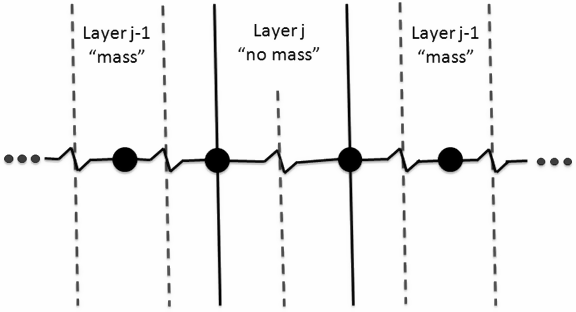
\includegraphics[width=0.9\textwidth, height=0.9\textheight, keepaspectratio=true]{media/image172.png}
\caption{Illustration of no-mass layer between two mass layers \protect \label{fig:illustration-of-no-mass-layer-between-two}}
\end{figure}

From the EnergyPlus code, the A matrix (AMat) is assigned with values at the interface using the following equations (taken from the actual code):

\begin{lstlisting}
cap = ( rho(Layer)\*cp(Layer)\*dx(Layer) + rho(Layer+1)\*cp(Layer+1)\*dx(Layer+1) ) \* 0.5D0
AMat(Node,Node-1) = rk(Layer)/dx(Layer)/cap           ! Assign matrix values for the current node
AMat(Node,Node)   = -1.0D0 \* ( rk(Layer)/dx(Layer)+rk(Layer+1)/dx(Layer+1) ) / cap
AMat(Node,Node+1) = rk(Layer+1)/dx(Layer+1)/cap       ! node.
\end{lstlisting}

Note that these equations do not change.~ For ``no mass'' layers, the density (rho) and the specific heat (cp) variables will be assigned zero values.~ In addition, the thickness (dx) will be equated with the user-defined R-Value and conductivity (rk) will be assigned a value of unity.~ In addition, the number of nodes for the ``no mass'' layer will be set to 1.

This handles resistive layers correctly without resorting to assigning the properties of air to the ``no mass'' layer.~ The only potential problem with this is if two resistive layers are placed next to each other.~ In that case, the interface between the two resistive layers would have no mass (variable ``cap'' would equal zero) and a divide by zero would result.~ To avoid this, adjacent ``no mass'' layers are combined internally so that the user does not have to do this and also to avoid any divide by zero errors.

While from a results standpoint, the difference in output between assigning air properties for specific heat, density, etc. and handling the no mass materials explicitly is negligible, handling the no mass layers properly does provide better code efficiency from a calculation speed standpoint.

\subsection{References}\label{references-014}

Ceylan, H. T., and G. E. Myers. 1980. Long-time Solutions to Heat Conduction Transients with Time-Dependent Inputs. ASME Journal of Heat Transfer, Volume 102, No. 1, pp.~115-120.

Hittle, D. C. 1979. Calculating Building Heating and Cooling Loads Using the Frequency Response of Multilayered Slabs, Ph.D.~Thesis, University of Illinois, Urbana, IL.

Hittle, D. C., and R. Bishop. 1983. An Improved Root-Finding Procedure for Use in Calculating Transient Heat Flow Through Multilayered Slabs. International Journal of Heat and Mass Transfer, Vol. 26, No. 11, pp.~1685-1693.

Ouyang, K., and F. Haghighat. 1991. A Procedure for Calculating Thermal Response Factors of Multi-layered Walls--State Space Method. Building and Environment, Vol. 26, No. 2, pp.~173-177.

Seem, J. E. 1987. Modeling of Heat Transfer in Buildings, Ph.D.~Thesis, University of Wisconsin, Madison, WI.

Strand, R. K. 1995. Heat Source Transfer Functions and Their Application to Low Temperature Radiant Heating Systems, Ph.D.~Thesis, University of Illinois, Urbana, IL.

Taylor, R. D., C.O. Pedersen, D.E. Fisher, R. J. Liesen, L.K. Lawrie. 1990. \emph{Simultaneous Simulation of Buildings and Mechanical Systems in Heat Balance Based Energy Analysis Programs}, Proceedings of the 3rd International Conference on System Simulation in Buildings, Liege, Belgium, December 3-5, 1990.

Taylor, R.D., C.O. Pedersen, D.E. Fisher, R. J. Liesen, L.K. Lawrie. 1991. Impact of Simultaneous Simulation of Buildings and Mechanical Systems in Heat Balance Based Energy Analysis Programs on System Response and Control, Conference Proceedings IBPSA Building Simulation '91, Nice, France, August 20-22, 1991.
